%=========================================================
\chapter{Avances Realizados}	
\label{cap:reqSist}

	En este capítulo se modela la {\em Arquitectura del negocio} la cual está conformada por la Ontología del negocio ({\em Términos} y {\em Hechos del negocio}), Arquitectura de procesos y las {\em Reglas del negocio}. Primero se especifica brevemente el {\em Contexto} en el que los términos tienen significado.
	
	En las secciones \ref{sec:terminosDeNegocio} y \ref{sec:hechosDeNegocio} se presentan los Términos del negocio a manera de Glosario y por último se presentan los Hechos del negocio a manera de relaciones entre términos del negocio.

%----------------------------------------------------------
\section{Iteración 1}
\subsection{Arquitectura}


\begin{figure}[htbp!]
	\begin{center}
		\fbox{\includegraphics[width=.6\textwidth]{images/Arquitectura}}
		\caption{Arquitectura del sistema.}
		\label{fig:Arquitectura}
	\end{center}
\end{figure}
\subsection{Búsqueda del framework para el desarrollo del proyecto} 
Se hizo una investigación sobre diversas herramientas para el desarrollo del proyecto, entre las cuales se puede incluir Spring MVC y Struts. 

Durante la investigación, y estudio de las mismas se hicieron diversas pruebas, que simulan el funcionamiento del proyecto. 

Las pruebas buscaban que se pudieran cargar aplicaciones externas, para el desarrollo del proyecto, ver el tiempo y dificultad requerido para capacitar a los demás miembros del equipo. Ver las ventajas que nos ofrecía para el desarrollo del mismo entre otros. 
\subsection{Diseño de la base de datos}
Se modeló la base de datos de acuerdo a los datos históricos de mayor relevancia que serían útiles para la toma de decisiones. Sin embargo, para ello se tuvo que hacer una pausa sobre su planeación. Donde se incluye una investigación, sobre la toma de decisiones, y la clasificación. Haciendo uso de reconocimiento de patrones y minería de datos, tomando los conceptos más importantes, así como las técnicas que se utilizan, para finalizar con el diseño de la base de datos. 

La base de datos se generó respectivamente con las labores de análisis sobre el negocio que se tendrá en la aplicación desde la creación de proyectos, la configuración de tareas, la invitación de colaboradores, la asignación de tareas. 

Cada una de las tablas creadas se basaron conforme a los negocios anteriormente mencionados, se crearon las respectivas relaciones entre tablas, se definieron los tipos de datos de las columnas, los id que serían auto incrementales, y finalmente el diagrama quedó de la siguiente forma: 

\begin{figure}[htbp!]
	\begin{center}
		\fbox{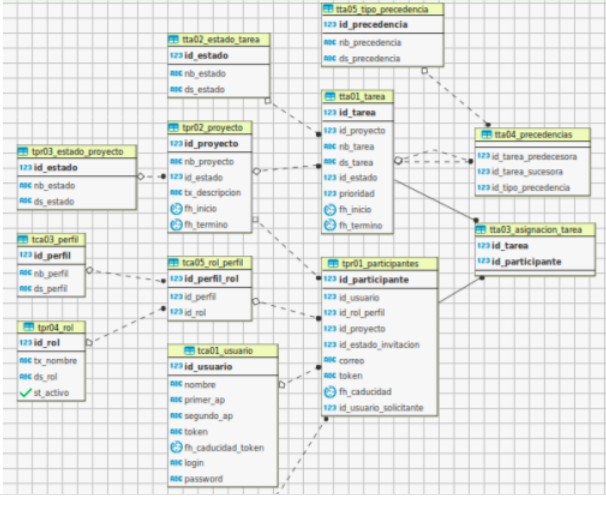
\includegraphics[width=.6\textwidth]{images/BaseDatos}}
		\caption{Diseño de la base de datos.}
		\label{fig:BaseDatos}
	\end{center}
\end{figure}

%----------------------------------------------------------
\section{Iteración 2} 
\subsection{Realización de mockups }
Se inició con un prototipo base de los datos que tendría que tener cada pantalla, desde su inicio hasta parte de su funcionamiento. Cada mockup refleja la relación que tiene una pantalla con respecto a otra. Durante el diseño hubo muchos cambios, pues debido a que el sistema contempla, desde la visualización de diversas herramientas, otras desaparecen y quedan inaccesibles dependiendo del rol del usuario. Entre las vistas consideradas están;  
Crear un proyecto, Crear una tarea, visualizar una tarea, visualizar la información de un proyecto, datos estadísticos, entre otras

En el caso de que uno sea líder o coordinador las acciones disponibles cambian, de igual forma estas dependen también del estado del proyecto. 

\subsection{Ambiente de Desarrollo } 

El entorno de trabajo se estableció de acuerdo a que se seleccionó como framework struts2, por lo cual se necesitó de primera instancia instalar un ide para poder codificar para este framework basado en java. Dicha ide fue eclipse, la cual nos facilita la implementación del proyecto con la utilización del framework.  
\begin{figure}[htbp!]
	\begin{center}
		\fbox{
\includegraphics[width=.6\textwidth]{images/eclipse}}
	\end{center}
\end{figure}
\newline \newline
Una vez seleccionada la ide prosiguió a seleccionar un gestor de base de datos, para el proyecto se seleccionó postgresql en el cual se montaría la base de datos del proyecto. Respectivamente se instaló y se creó una base de datos en blanco. 
\newline \newline
A su vez seleccionado el gestor de base de datos, para poder facilitar el trabajo de creación de tablas, y generación de queries se utilizó un ide para poder realizar acciones en la base de datos generada en postgres dicha herramienta fue dbeaver, el cual facilita el trabajar la base de datos con una interfaz gráfica fácil de dominar.
\newline \newline
\begin{figure}[htbp!]
	\begin{center}
		\fbox{
\includegraphics[width=.6\textwidth]{images/DBeaver}}
		\caption{DBeaver}
		\label{fig:DBeaver}
	\end{center}
\end{figure}

Y finalmente la herramienta que se seleccionó para subir los cambios al repositorio donde se montó el proyecto, gitKraken herramienta utilizada para realizar las acciones básicas de un repo git los cuales serían commits, push, pull, fetch.
\newline \newline
Esas fueron las herramientas instaladas como ambiente de desarrollo para la generación del proyecto. Dichas herramientas fueron seleccionadas ya que se adecuaron para la forma de trabajo para la metodología seleccionada. 

Con ello generado el proyecto se prosiguió a colocar la configuración del framework la cual consto de 4 archivos los cuales son: 
\newline \newline
applicationContext.xml 
\newline \newline
En este archivo se compilan el resto de xml los cuales conllevan los parámetros de configuración para el pool de conexiones, los datos para la generación de la conexión mediante jpa y la toma en cuenta de los mapeos para dicha conexión con la base de datos, el nombre base para los paquetes que incluirán las clases para los actions, bs, y dao del proyecto.  
\newline \newline
dataSource.xml 
\newline \newline
Este archivo contiene los parámetros del bean que se encargará de la conexión de la base de datos, así como los datos del pull de dicha conexión, con esto se conlleva también a la creación del entitymanager. 
\newline \newline
hibernateSessionFactory.xml 
\newline \newline
En este xml se define en dialecto se trabajarán las consultas a la base de datos, que para este caso fue el dialecto para postgresql, tambien se definio en que package se guardan las clases que representan a las tablas en la base de datos. 
\newline \newline
 struts.xml 
\newline \newline
Archivo de configuración del framework el cual contiene desde la configuración regional e idioma del proyecto, así como definición de los interceptores, filtros y listeners, archivos de datos como los properties variables que se utilizarían en cualquier parte del proyecto, y cuestiones como la convención de directorios de url utilizado en este caso REST, entre otras configuraciones. 

%----------------------------------------------------------
\section{Iteración 3} 

\subsection{Programación de la GUI del sistema } 

 Se procedió a utilizar como referencia a los mockups del sistema que se habían hecho previamente para ello se generó un proyecto que se llamó en maquetado, en el cual se puso todas las pantallas del proyecto que se contemplaron para la primera fase del proyecto (TT1), donde dicho proyecto de en maquetado, tendría como único objetivo mostrar un prototipo del proyecto en cuanto a navegación. La programación del mismo permitió que se arreglaran los errores de diseño que no habían sido contemplados en un inicio. 

Para la programación de la GUI del sistema se utilizó bootstrap permitiendo con ello hacer que fuera su diseño responsivo. Ahorrando horas de programación. Así mismo agregando diversas funcionalidades extras al sistema. 

Dentro de la programación se agregaron las gráficas que se habían hecho en Chart.js y en paper.js, para tener una idea más clara de lo que sería el producto final.


\subsection{Pruebas de la navegación de GUI de sistema}
Una vez programada la navegación del sistema, se procedió a hacer pruebas para determinar posibles errores que pudiera haber con el framework y el mismo sistema. 


En este punto se procedió a trasladar la mayor parte de lo que se había hecho en el proyecto de en maquetado. agregando funcionalidad a todo el proyecto. Tanto a las gráficas como a cada proceso dentro de la creación de un proyecto. dría la estructura de carpetas que conforman a un proyecto web. 
 

Para acceder previamente se debió de crear una cuenta en el sistema la cual es el correo electrónico y registro de un password para dicho correo. Ya que se tienen la cuenta se ingresan los datos, el sistema valida que dicho usuario esté en la base de datos y en caso afirmativo puedes entrar a la pantalla principal del sistema, en caso contrario recibirás un mensaje de error el cual te dirá que el usuario y/ contraseña son incorrectos. 

%----------------------------------------------------------	
\section{Iteración 4}
\subsection{Análisis y programación del Módulo de control de acceso}

Se analizo los requerimientos y reglas de negocio necesarias para la implementación del login de la aplicación, el registro de los usuarios y la recuperación de las contraseñas de las cuentas de los usuarios. 

Siendo primero el Loguin se programó como es debido solicitando los datos de su correo y contraseña validando que primero que exista el usuario, si existe se verifica que el password coincida con el otorgado, una vez verificado que sea el mismo se otorga el acceso al sistema. Se realizaron las pruebas para corroborar que el login funcionase y se mostró dicho funcionamiento. 

Una vez terminando el login se creó el registro de los usuarios, tomando en cuenta validaciones como que el correo a registrar no exista en el sistema, y que se introduzca un correo electrónico valido, longitudes de capo máximo a 100, cumpliendo dichas validaciones el usuario ya posee una cuenta en el sistema.  

Como pruebas se verifico que al crearse la cuenta se pudiera efectivamente entrar a la aplicación, una vez realizada la prueba y obteniendo resultados positivos se programó la recuperación de cuenta. 

Para la recuperación de cuenta se utilizó la interfaz solicitando el correo de la cuenta que se necesita recuperar, dando le click se generó un correo el cual constaba de un enlace para el cambio de la contraseña, para efectuar el cambio en el URL se pasó la cuenta y un token el cual deban coincidir con lo registrado en la base si tanto la cuenta junto con el toen no coincidían se arroja un mensaje de error, en caso contrario se permite el cambio de contraseña de la cuenta. 

Con lo anterior se culminó la programación del módulo de control de acceso.

%---------------------------------------------------------
\section{Iteración 5}
\subsection{Análisis y programación del Módulo de registro de proyectos.}

De manera similar se analizaron los requerimientos para el módulo de proyectos, obteniendo las validaciones y reglas de negocio que involucra la gestión de un proyecto. 

Se programo un CRUD el cual constaba de la creación del proyecto, teniendo en cuenta datos como el nombre del proyecto, el autor que lo crea, la duración de proyecto (fechas de inicio y termino), y una descripción de lo que el autor quiera mostrar o más bien decir sobre que trata el proyecto que creo. 
 

Se programo la edición del proyecto la cual permite modificar los parámetros antes mencionados para la creación dándole la oportunidad al usuario en caso de equivocarse. De igual forma se generó el visualizado de los datos generales del proyecto siendo los mismos parámetros con los que se crea los que se mostraron en texto solo dando la información del proyecto. 

Y finalmente la búsqueda la cual el componte “dataTable” la otorga dejando un input en el cual deja introducir lo que se está buscando en particular en este caso un proyecto. 

Como el módulo anterior se realizaron pruebas para determinar que el módulo de gestión de proyectos esté funcionando de manera en la que se analizó, se obtuvieron pruebas positivas. 

%---------------------------------------------------------
\section{Iteración 6}
\subsection{Análisis y programación del módulo de gestión de tareas.}

El módulo de gestión de tareas, se analizó y tardo más en su programación, se tomaron en consideración más factores en los que se involucran en este módulo desde el CRUD de las tareas, así como la relaciones que se darán entre tareas, y como reflejar dichas tareas en un diagrama de gantt, junto con las relaciones. 

Comenzando por analizar el módulo de tareas consto de un CRUD el cual inicio con el registro de tareas, se solicitaron datos como un nombre, fechas de inicio y fechas de fin, los campos anteriores teniéndose en cuenta dos casos de registro una en periodos y otra en días, la primera dando una fecha de inicio y una de fin, y la segunda teniendo como inicio el día actual y dependiendo los días introducido se determinara una fecha de fin. 

De manera similar como anteriores CRUD se programó la edición de las tareas creadas, así como se creó una vista para los datos generales de la misma, de igual forma se pueden eliminar las tareas, pero con la condición de que estas no tengan un avance registrado. Lo anterior mencionado se puede tomar como la gestión de tareas. 

En la misma pantalla de gestión de tareas se colocaron en la vista tres tabs lo cuales un es para la misma gestión de tareas, el segundo para mostrar el diagrama de gantt el cual mostrara todas las tareas del proyecto, viendo una tarea general que es la fecha en la que dura el proyecto, y las consecuentes serán las tareas que se registraron para el mismo proyecto. 

Siguiendo con el gantt, para generarlo se utilizó el api de google para la creación de charts, entre ellos se incluía el gantt se implementó en la aplicación, siguiendo la documentación dada por la misma compañía. Al gantt se le creo un JSON con la lista de tareas pertenecientes al proyecto en gestión, teniendo encuentra la estructura marcada en la documentación para crear cada elemento referente a una tarea del proyecto. 

Como datos a mostrar en el gantt se puede visualizar al pasar por cada tarea un pequeño globo de información la cual incluye la fecha de inicio la fecha de término, el porcentaje de avance, y quienes son os asignados a dicha tarea. 

La siguiente pestaña es la de estadística en la cual se ve un grafica de barras la cual representa las horas trabajadas, las horas que faltan por trabajar, el retraso de la realización de las tareas. Esto con el fin de que el líder de proyecto tenga encuentra quien está asignado a la tarea, así como el avance que llevan todo los involucrados en la tarea. Lo anterior representa lo realizado para la iteración. 

%---------------------------------------------------------
\section{Iteración 7}
\subsection{Continuación Desarrollo módulo de gestión tareas.}

Lo siguiente fue el desarrollo de las dependencias entre tareas a cuáles constan de cuatro tipos los cuales son: 

Fin-Inicio: la actividad siguiente B no puede empezar hasta que no haya terminado la actividad precedente A. 

Inicio-inicio: la actividad siguiente B puede empezar una vez que haya comenzado la actividad precedente A. 

Fin-Fin: la actividad siguiente B puede finalizar cuando haya finalizado la precedente A. 

Inicio-Fin:  La actividad B no puede terminar hasta que no haya acabado la actividad A. 

Estas dependencias se guardan y validan para que concuerden con las fechas en la que se registró la tarea, y no se almacén solo por almacenar, una vez registradas podemos regresar a la pantalla en al que se registraron las dependencias ahí observaremos las dependencias que tiene nuestra tarea con otras, una vez yendo a la pestaña del gantt se verán reflejadas las dependencias.  

%---------------------------------------------------------
\section{Iteración 8}
\subsection{Análisis y Desarrollo del módulo de Invitación y asignación de colaboradores.}


%---------------------------------------------------------
\section{Iteración 9}
\subsection{Análisis y Desarrollo del moduló de reporte de avances.}

En este módulo se analizó que es lo que los colaboradores subirían como avances en el sistema. Se dividieron en dos casos uno en el que el programador como avance reportaría el número de commit y atreves de un api se calcularían las líneas de código que programo para dicho commit, esto serviría para alimentar a nuestro sistema a la hora de las sugerencias de colaboradores en el rol de programador, para el rol de analista se utilizó como alimentación cuantos veces reportan avance de documentación a través del versionamiento en drive de google, para ello el colaborador introduce u n enlace referente a un documento almacenado en drive y atreves de dicho versionamento se sabrá si es que se modificó o no. 

Para reportar los avances se analizó y programo de tal manera en que el líder en primera instancia tiene que registrar el repositorio en git en la que montara el proyecto y a su vez en la que sus colaboradores subirán sus avances. Lo anterior se realiza en a tabla de gestión de proyectos siempre y cuando seas el dueño y con rol de líder de proyecto, podrás registrar el url del proyecto, para la documentación drive no necesitas dar el url del documento. 

Para que los colaboradores puedan reportar su avance en la misma pantalla de gestión de proyecto en el caso de ser colaborador te aparecerá otra pantalla la cual será una gestión de las tareas que se te hayan asignado, una vez dentro de la gestión se seleccionara el icono para el reporte de avances una vez dentro la pantalla te mostrara un los datos generales de la tarea como a fecha en la que inicia y la fecha en la que debe terminar, así como chart que muestra el avance reportado por el colaborador, para dicho reporte habrá un icono con el logo de play el cual a presionar comenzara a tomar en cuenta el tiempo en el que se está elaborando la tarea y cada vez que el usuario ponga en pausa la área se pedirá que reporte el avance que lleva dado por un cadena que representa al commit en git y otro campo que representa el porcentaje que el usuario considere que lleva avanzado. Cada vez que lo haga se registrara el avance hasta alcanzar la totalidad de la tarea. 

A su vez que se reportan avances en el char se arroja una estimación de cuánto tiempo le tomara al usuario terminar la tarea. 


%---------------------------------------------------------


